% ==============================================================================
% PLANTILLA MAESTRA - ETICA Y MORAL JURIDICA / UnADM
% ==============================================================================
% Uso:
% 1. Duplica este archivo y renombra la copia por semana/actividad.
% 2. Actualiza documenttitle, documentsubtitle y documentsubject.
% 3. Lee la planeacion semanal y NO pegues las instrucciones completas dentro del
%    producto final. Usa la planeacion como lista de cumplimiento.
% 4. Consulta la bibliografia indicada por la docente, toma notas y redacta con
%    criterio propio: concepto -> caracteristicas -> funcion juridica -> postura.
% 5. Entrega en PDF con la nomenclatura indicada en el aula.
%
% Objetivo general de la asignatura:
% - Comprender las bases eticas y las relaciones morales del Derecho.
%
% Objetivos especificos recurrentes en las planeaciones:
% - Identificar las principales escuelas de etica relacionadas con el Derecho.
% - Reconocer las implicaciones de la moral en el ambito juridico.
% - Relacionar etica y moral en el contexto social.
% - Analizar derechos y dignidad humana en el contexto juridico.
%
% Formato institucional aplicado:
% - Fuente tipo Helvetica, equivalente visual a Arial.
% - Interlineado 1.5.
% - Citas autor-anio con natbib: usar \citep{clave} o \citet{clave}.
% - Referencias en bibliografia BibTeX, formato APA 7 en cuerpo y referencias.
% - Redaccion academica, clara, con analisis propio y buena ortografia.
% - Caratula, desarrollo, conclusion y bibliografia.
%
% Regla para productos visuales:
% - Si la actividad pide tabla, cuadro comparativo, esquema, mapa conceptual,
%   mapa mental, linea de tiempo, diagrama, matriz, red conceptual, SQA,
%   organizador grafico o producto similar, realizarlo preferentemente con
%   LaTeX/TikZ para mantener nitidez, evidencia editable y diseno controlado.
% - Si se usa Canva, Miro u otra plataforma, insertar capturas nitidas y conservar
%   evidencia suficiente dentro del PDF.
%
% Criterios derivados de la evaluacion recibida en Etica y Moral juridica:
% - Plantea conceptos precisos: 3 puntos.
% - Menciona caracteristicas con claridad: 3 puntos.
% - Presenta buena redaccion y ortografia: 2 puntos.
% - Usa fuentes, citas y referencias en formato APA 7: 2 puntos.
%
% Criterios de Semana 3 detectados en planeacion:
% - Realiza un formato correcto.
% - Utiliza contenido filosofico puro cuando la actividad lo solicite.
% - Integra criticas pertinentes, no solo definiciones.
% - Mantiene redaccion clara y referencias APA 7.
%
% Criterios de redaccion personal (enfoque aplicado):
% - No escribir para llenar espacio; escribir para sostener una idea.
% - Cada concepto debe responder: que es, que caracteristicas tiene, como
%   funciona, que problema resuelve, que limite presenta y que implicacion
%   juridica tiene.
% - Evitar listas sin analisis. Despues de cada dato importante, explicar su
%   consecuencia.
% - Estructura mental recomendada: problema etico -> criterio moral -> efecto
%   juridico -> postura personal.
% - Usar primera persona con moderacion academica: "Considero que",
%   "Desde esta perspectiva", "La posicion que sostengo es". Evitar "yo creo".
%
% Productos recurrentes segun planeaciones de la materia:
% - Semana 2: Cuadro comparativo.
% - Semana 3: Esquema.
% - Semana 4: Linea de tiempo.
% - Semana 5: Mapa conceptual.
% - Semana 6: Resumen.
% - Semana 7: Reporte de lectura general.
% - Semana 8: Analisis de hechos.
% - Semana 9: Ensayo.
%
% Checklist antes de entregar:
% [ ] El objetivo coincide con la planeacion de la semana.
% [ ] El producto solicitado aparece de forma visible y bien rotulada.
% [ ] Los conceptos son precisos y no se contradicen.
% [ ] Las caracteristicas estan explicadas con claridad, no solo enumeradas.
% [ ] Hay citas APA autor-anio dentro del texto.
% [ ] Hay bibliografia al final y coincide con las fuentes citadas.
% [ ] La introduccion plantea una idea propia, no solo anuncia la actividad.
% [ ] La conclusion responde que se comprendio y que postura se sostiene.
% [ ] No aparecen instrucciones copiadas de la planeacion dentro del producto.
% [ ] Si se uso IA como apoyo, el texto fue comprendido, revisado y apropiado.
% ==============================================================================

% CREACION DEL DOCUMENTO
\documentclass[
	spanish,
	letterpaper, oneside
]{article}

% ==============================================================================
% INFORMACION DEL DOCUMENTO
% Actualizar en cada actividad.
% Ejemplos:
% \def\documenttitle {Cuadro comparativo de escuelas clasicas de la etica}
% \def\documentsubtitle {Actividad 2 - Etica y Moral juridica}
% \def\documentsubject {Actividad Semana 2}
% ==============================================================================
\def\documenttitle {Relación entre moral y Derecho en el ámbito jurídico mexicano}
\def\documentsubtitle {Actividad 4 - Ética y Moral jurídica}
\def\documentsubject {Semana 5 - Etica y Moral jurídica}

\def\documentauthor {Martín Jonathan de la Cruz}
\def\coursename {Ética y Moral jurídica}
\def\coursecode {030}

\def\universityname {Universidad Abierta y a Distancia de México}
\def\universityfaculty {Licenciatura en Derecho}
\def\universitydepartment {Ética y Moral jurídica}
\def\universitydepartmentimage {departamentos/UnADM}
\def\universitydepartmentimagecfg {height=1.57cm}
\def\universitylocation {Roma Norte, Ciudad de México}

% INTEGRANTES, PROFESORES Y FECHAS
\def\authortable {
	\begin{tabular}{ll}
		\textbf{Alumno:}
		& \begin{tabular}[t]{l}
			 Martín Jonathan de la Cruz \\
		\end{tabular} \\
		Matrícula: & ES2611202040 \\

		\textit{Profesor:}
		& \begin{tabular}[t]{l}
			Emma Liliana \\ Padilla Cano
		\end{tabular} \\
		& \\
		\multicolumn{2}{l}{Fecha de realización: \today} \\
		\multicolumn{2}{l}{\universitylocation}
	\end{tabular}
}

% IMPORTACION DEL TEMPLATE
\input{template}

% FORMATO SOLICITADO / USADO EN ACTIVIDADES CORREGIDAS
\usepackage{helvet}
\renewcommand{\familydefault}{\sfdefault}

% PRODUCTOS VISUALES EN TIKZ
\usepackage{tikz}
\usetikzlibrary{
	arrows.meta,
	positioning,
	calc,
	matrix,
	fit,
	shapes.geometric,
	shadows.blur
}

% ==============================================================================
% MARCA DE AGUA (adaptada de Plantilla - UnADM)
% - Para apagarla: \def\coverwatermarkenabled {false}
% ==============================================================================
\def\coverwatermarkenabled {true}
\def\coverwatermarkimage {img/departamentos/UnADM.pdf}
\def\coverwatermarkopacity {0.16}
\def\coverwatermarkwidth {0.72\paperwidth}
\def\coverwatermarkxshift {0cm}
\def\coverwatermarkyshift {-0.35cm}

\newcommand{\insertcoverwatermark}{%
	\ifthenelse{\equal{\coverwatermarkenabled}{true}}{%
		\AddToShipoutPictureBG*{%
			\begin{tikzpicture}[remember picture,overlay]
				\node[
					opacity=\coverwatermarkopacity,
					inner sep=0pt,
					xshift=\coverwatermarkxshift,
					yshift=\coverwatermarkyshift
				] at (current page.center) {%
					\includegraphics[width=\coverwatermarkwidth]{\coverwatermarkimage}%
				};
			\end{tikzpicture}%
		}%
	}{}%
}

% CITAS EN FORMATO AUTOR-ANIO, COMPATIBLE CON APA 7 EN EL CUERPO DEL TEXTO
% Usar:
% - Cita parentetica: \citep{clave}
% - Cita narrativa: \citet{clave}
% - Varias fuentes: \citep{clave1,clave2}
\setcitestyle{authoryear,open={(},close={)}}

% ==============================================================================
% AYUDAS DE REDACCION
% Quitar o comentar \pendiente cuando el documento final este terminado.
% ==============================================================================
\newcommand{\pendiente}[1]{\textcolor{red}{[PENDIENTE: #1]}}

\begin{document}

% PORTADA
\insertcoverwatermark
\templatePortrait

% CONFIGURACION DE PAGINA Y ENCABEZADOS
\templatePagecfg
\onehalfspacing

% ==============================================================================
% RESUMEN / ABSTRACT
% Debe ser breve, no copiar instrucciones.
% Formula recomendada:
% Tema + objetivo + tecnica/producto + enfoque personal.
% ==============================================================================
\begin{abstractd}
	\textbf{Objetivo:} Analizar, mediante un mapa conceptual, cómo se relacionan la moral y el Derecho en el ámbito jurídico mexicano.

	\textbf{Producto elaborado:} Mapa conceptual con cuatro ramas: moral, Derecho, relación entre ambos y autores.

	\textbf{Enfoque de análisis:} Tomo el tema como un sistema de control: la moral aporta criterios de valoración y el Derecho aporta forma, procedimiento y fuerza institucional. El punto delicado está en no confundir moral crítica con imposición de moral privada.
\end{abstractd}

% TABLA DE CONTENIDOS - INDICE
\templateIndex

% CONFIGURACIONES FINALES
\templateFinalcfg

% ======================= INICIO DEL DOCUMENTO =======================

% ==============================================================================
% SECCION 1: INTRODUCCION
% Apertura recomendada:
% - Iniciar con una afirmacion fuerte.
% - Traducir la consigna a problema etico-juridico.
% - Mostrar por que el tema importa para la formacion juridica.
% - Cerrar anticipando el enfoque personal.
%
% Evitar:
% - "En este trabajo hablare de..."
% - "La etica es muy importante..."
% - Definiciones de diccionario sin interpretacion.
% ==============================================================================
\section{Introducción}

La relación entre moral y Derecho no puede tratarse como una simple definición. El problema real es más práctico: una norma puede estar escrita correctamente y, aun así, producir una decisión injusta si se aplica sin criterio. También puede pasar lo contrario: una idea moral puede parecer correcta para una persona, pero no por eso debe imponerse como obligación jurídica.

Desde esa idea organicé el mapa conceptual. El centro es la relación entre moral y Derecho en México; alrededor se ubican las ramas que permiten entender el sistema: qué es la moral en el campo jurídico, cómo funciona el Derecho, dónde se cruzan ambos y qué aportan algunos autores mexicanos o vinculados con la reflexión ética en México.

Considero que el Derecho necesita moral, pero no cualquier moral. Necesita una moral que pueda convertirse en razón pública: dignidad, justicia, igualdad, responsabilidad y límites al poder. Si no existe ese filtro, la moral puede volverse imposición; pero si el Derecho se queda sin moral crítica, corre el riesgo de volverse puro trámite.

% ==============================================================================
% SECCION 2: DESARROLLO / ANALISIS
% Organizar segun el producto solicitado:
% - Cuadro comparativo: escuela/concepto, definicion, caracteristicas,
%   fundamento, pregunta clave, critica, autor y aplicacion juridica.
% - Esquema: concepto central, ramas principales, notas de funcion y limites.
% - Linea de tiempo: periodo, autor, escuela, aporte, consecuencia etica/juridica.
% - Mapa conceptual: conceptos unidos por conectores verbales claros.
% - Resumen: tesis central de la lectura, argumentos, conceptos y cierre personal.
% - Reporte de lectura: ficha, objetivo, ideas centrales, analisis y valoracion.
% - Analisis de hechos: hechos, problema etico, criterios, valoracion, postura.
% - Ensayo: tesis, argumentos, contraargumento, postura y conclusion.
%
% Regla de parrafo:
% Entrada: concepto o problema.
% Proceso: explicacion, fuente y relacion.
% Salida: consecuencia etica, moral o juridica.
% ==============================================================================
\section{Mapa conceptual: moral y Derecho en México}

En el ámbito jurídico conviene separar tres formas de moral. La moral personal pertenece a la conciencia individual. La moral social positiva refleja costumbres y valores compartidos. La moral ideal o crítica sirve para preguntar si esas costumbres son justas o si deben cambiar. Esta distinción evita un error común: pensar que toda costumbre social ya es correcta sólo porque muchas personas la aceptan \citep{ronquilloarmasEticaGeneralProfesional2018,singerCompendioEtica1995}.

El Derecho trabaja con otra lógica: norma, obligación, sanción y procedimiento. García Máynez ayuda a ver la diferencia entre legalidad y moralidad: cumplir la forma legal no siempre agota el problema ético \citep{garciaMaynezEtica}. Para mí, ahí está el punto útil de la actividad: una decisión jurídica no debe limitarse a aplicar un texto; debe justificar por qué esa aplicación respeta dignidad, justicia y derechos.

En México esta relación se nota en temas como dignidad humana, igualdad, debido proceso, daño moral, reparación integral y derechos humanos. No son adornos del discurso jurídico; funcionan como criterios para revisar si una autoridad está tratando a la persona como sujeto de derechos y no como simple expediente \citep{cndhMarcoNormativo2026}.

El límite es claro: la moral puede orientar la interpretación cuando se expresa como razón jurídica. Puede hablar de dignidad, igualdad, proporcionalidad o buena fe. Lo que no debe hacer es convertirse en censura o en imposición de una forma privada de vida.

\subsection{Análisis del mapa conceptual}

El mapa se lee desde el centro hacia afuera. La rama azul separa la moral en tres niveles: personal, social positiva e ideal crítica. Esta separación me parece necesaria porque ayuda a no confundir conciencia individual, costumbre social y criterio de justicia.

La rama verde muestra al Derecho como un sistema más formal: norma, obligación, sanción y justicia. Aquí la diferencia no está en que el Derecho no tenga valores, sino en que funciona mediante instituciones. Esa estructura le da fuerza, pero también exige control.

La rama naranja resume el cruce entre moral y Derecho. Se parecen porque ambos regulan conducta. Se distinguen porque el Derecho puede exigir y sancionar. Se limitan porque el Derecho no debe perseguir toda conducta moralmente discutible. Se encuentran cuando una norma se interpreta desde principios como dignidad, igualdad o proporcionalidad.

La rama roja integra autores que ayudan a sostener el análisis. García Máynez permite distinguir legalidad y moralidad; Sánchez Vázquez ubica la moral como fenómeno social; Villoro conecta valor, poder y legitimidad; y Juliana González refuerza la importancia de dignidad, libertad y responsabilidad \citep{garciaMaynezEtica,sanchezVazquezEtica1969,villoroPoderValor1997,gonzalezEthosDestino1996}.

Desde mi perspectiva, el mapa deja una idea central: el Derecho necesita forma legal, pero también necesita criterio. La forma evita arbitrariedad; el criterio evita que la norma se aplique como si las personas fueran sólo casos, expedientes o números. Esa es la diferencia entre aplicar una regla y razonar jurídicamente.

\clearpage
\pagestyle{empty}
\newgeometry{top=1.2cm,bottom=1.2cm,left=1.2cm,right=1.2cm}
\begin{landscape}
\thispagestyle{empty}
\begin{figure}[p]
\centering
\captionsetup{font=small,labelfont=bf}
\begin{adjustbox}{
	max width=0.96\linewidth,
	max totalheight=0.78\textheight,
	center
}
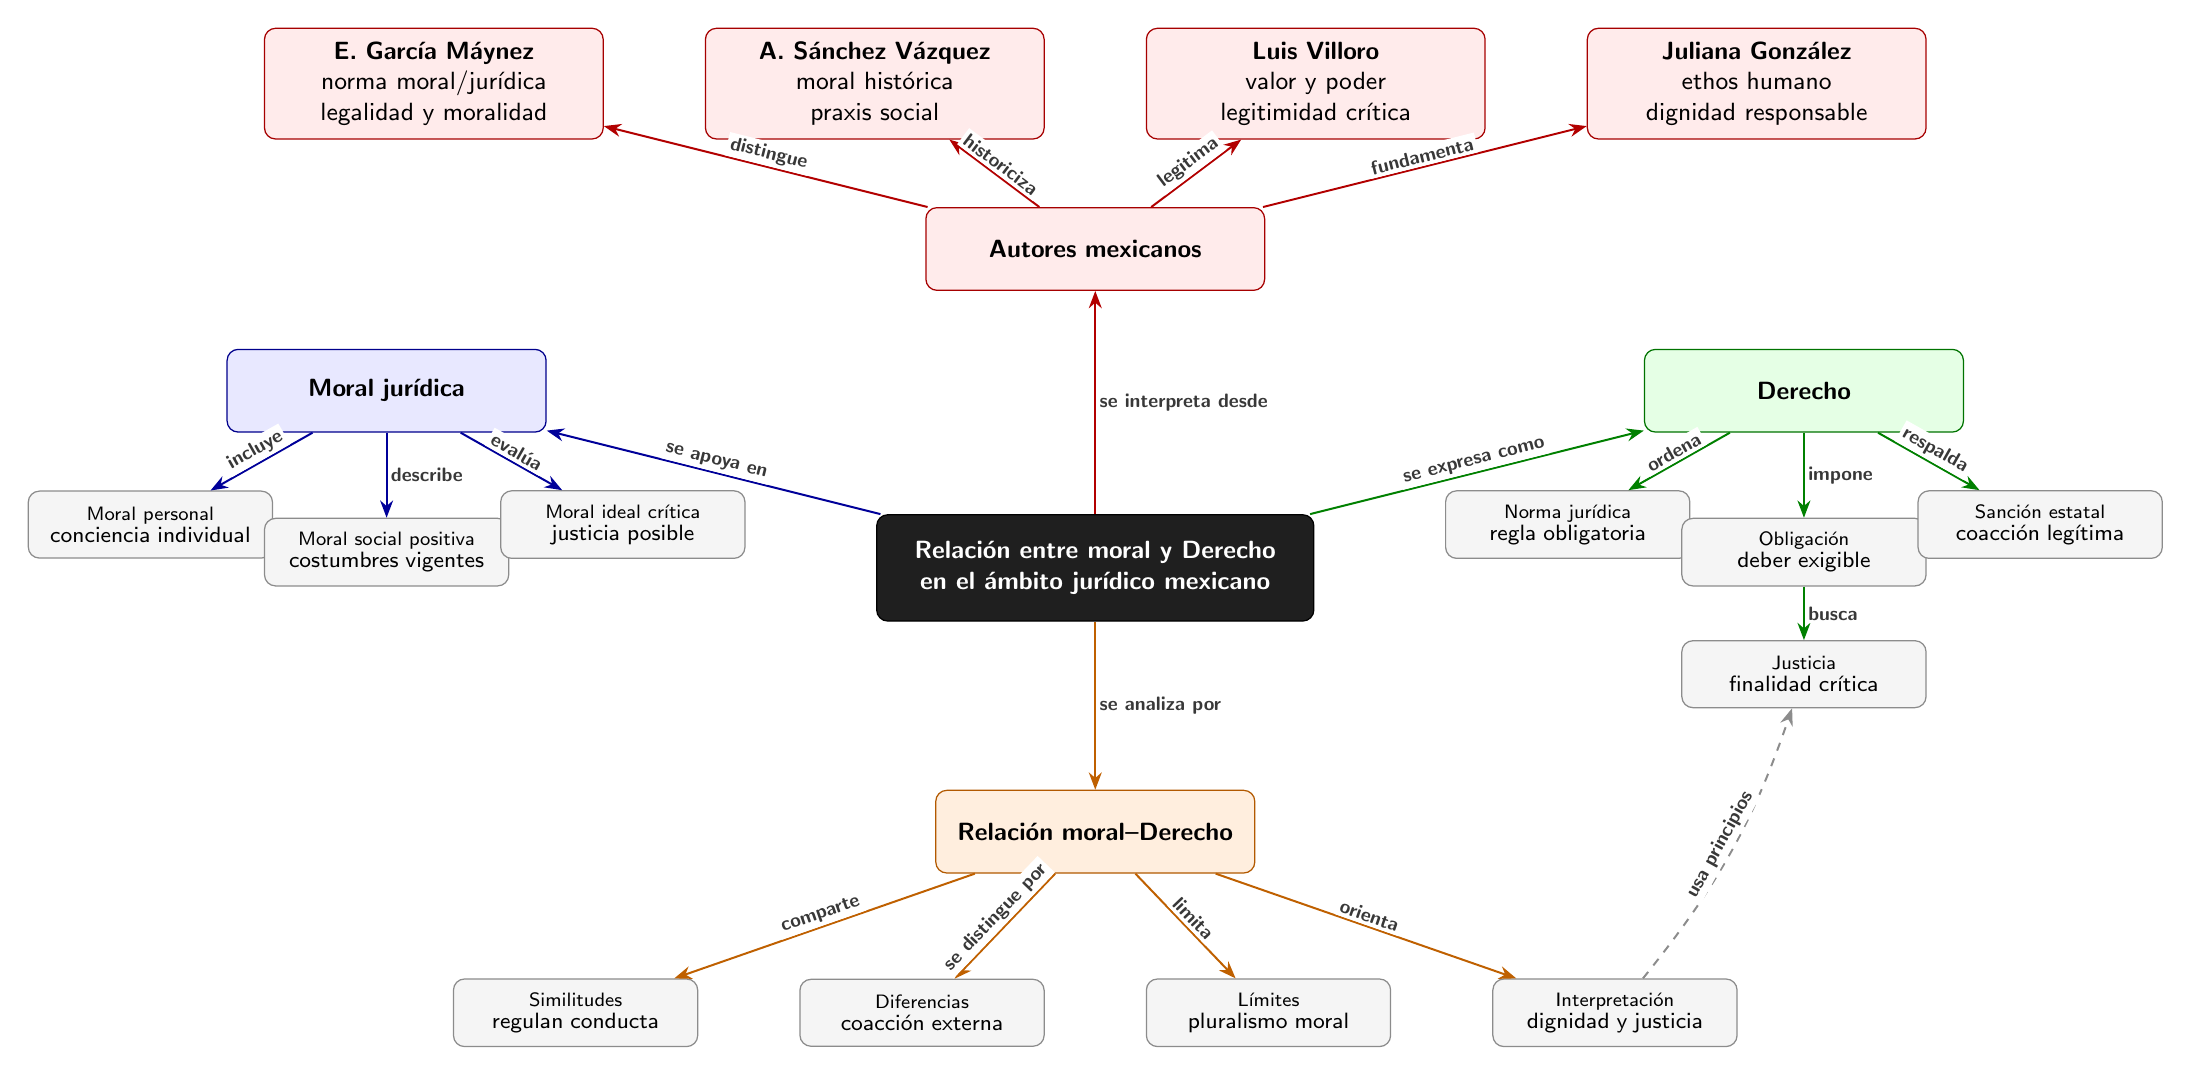
\begin{tikzpicture}[
	concept/.style={
		rectangle,
		rounded corners=4pt,
		draw=black!55,
		line width=0.45pt,
		align=center,
		text width=3.7cm,
		minimum height=1.05cm,
		inner sep=5pt,
		font=\small
	},
	root/.style={
		concept,
		fill=black!88,
		text=white,
		draw=black,
		text width=5.2cm,
		font=\bfseries\small,
		minimum height=1.35cm
	},
	moral/.style={concept, fill=blue!9, draw=blue!55!black},
	derecho/.style={concept, fill=green!10, draw=green!45!black},
	relacion/.style={concept, fill=orange!13, draw=orange!70!black},
	autor/.style={concept, fill=red!8, draw=red!65!black, text width=3.95cm},
	criterio/.style={concept, fill=gray!8, draw=black!45, text width=2.75cm, font=\scriptsize, minimum height=0.85cm},
	edge/.style={-{Stealth[length=2.2mm]}, line width=0.72pt, draw=black!60},
	label/.style={font=\scriptsize\bfseries, fill=white, inner sep=1.2pt, text=black!78}
]

\node[root] (centro) at (0,0) {Relación entre moral y Derecho\\en el ámbito jurídico mexicano};

% Ramas principales
\node[moral] (moral) at (-9,2.25) {\textbf{Moral jurídica}};
\node[derecho] (derecho) at (9,2.25) {\textbf{Derecho}};
\node[relacion] (rel) at (0,-3.35) {\textbf{Relación moral--Derecho}};
\node[autor] (autores) at (0,4.05) {\textbf{Autores mexicanos}};

\draw[edge, blue!60!black] (centro) -- node[label, above, sloped] {se apoya en} (moral);
\draw[edge, green!50!black] (centro) -- node[label, above, sloped] {se expresa como} (derecho);
\draw[edge, orange!75!black] (centro) -- node[label, right] {se analiza por} (rel);
\draw[edge, red!70!black] (centro) -- node[label, right] {se interpreta desde} (autores);

% Moral
\node[criterio] (mp) at (-12,0.55) {Moral personal\\\footnotesize conciencia individual};
\node[criterio] (msp) at (-9,0.2) {Moral social positiva\\\footnotesize costumbres vigentes};
\node[criterio] (mic) at (-6,0.55) {Moral ideal crítica\\\footnotesize justicia posible};

\draw[edge, blue!60!black] (moral) -- node[label, above, sloped] {incluye} (mp);
\draw[edge, blue!60!black] (moral) -- node[label, right] {describe} (msp);
\draw[edge, blue!60!black] (moral) -- node[label, above, sloped] {evalúa} (mic);

% Derecho
\node[criterio] (norma) at (6,0.55) {Norma jurídica\\\footnotesize regla obligatoria};
\node[criterio] (oblig) at (9,0.2) {Obligación\\\footnotesize deber exigible};
\node[criterio] (sancion) at (12,0.55) {Sanción estatal\\\footnotesize coacción legítima};
\node[criterio] (justicia) at (9,-1.35) {Justicia\\\footnotesize finalidad crítica};

\draw[edge, green!50!black] (derecho) -- node[label, above, sloped] {ordena} (norma);
\draw[edge, green!50!black] (derecho) -- node[label, right] {impone} (oblig);
\draw[edge, green!50!black] (derecho) -- node[label, above, sloped] {respalda} (sancion);
\draw[edge, green!50!black] (oblig) -- node[label, right] {busca} (justicia);

% Relaciones
\node[criterio] (sim) at (-6.6,-5.65) {Similitudes\\\footnotesize regulan conducta};
\node[criterio] (dif) at (-2.2,-5.65) {Diferencias\\\footnotesize coacción externa};
\node[criterio] (lim) at (2.2,-5.65) {Límites\\\footnotesize pluralismo moral};
\node[criterio] (interp) at (6.6,-5.65) {Interpretación\\\footnotesize dignidad y justicia};

\draw[edge, orange!75!black] (rel) -- node[label, above, sloped] {comparte} (sim);
\draw[edge, orange!75!black] (rel) -- node[label, above, sloped] {se distingue por} (dif);
\draw[edge, orange!75!black] (rel) -- node[label, above, sloped] {limita} (lim);
\draw[edge, orange!75!black] (rel) -- node[label, above, sloped] {orienta} (interp);
\draw[edge, black!45, dashed, bend right=10] (interp) to node[label, above, sloped] {usa principios} (justicia);

% Autores
\node[autor] (gm) at (-8.4,6.15) {\textbf{E. García Máynez}\\norma moral/jurídica\\legalidad y moralidad};
\node[autor] (sv) at (-2.8,6.15) {\textbf{A. Sánchez Vázquez}\\moral histórica\\praxis social};
\node[autor] (lv) at (2.8,6.15) {\textbf{Luis Villoro}\\valor y poder\\legitimidad crítica};
\node[autor] (jg) at (8.4,6.15) {\textbf{Juliana González}\\ethos humano\\dignidad responsable};

\draw[edge, red!70!black] (autores) -- node[label, above, sloped] {distingue} (gm);
\draw[edge, red!70!black] (autores) -- node[label, above, sloped] {historiciza} (sv);
\draw[edge, red!70!black] (autores) -- node[label, above, sloped] {legitima} (lv);
\draw[edge, red!70!black] (autores) -- node[label, above, sloped] {fundamenta} (jg);
\end{tikzpicture}
\end{adjustbox}
\caption{Mapa conceptual: relación entre moral y Derecho en el ámbito jurídico mexicano.}
\label{fig:mapa-moral-derecho}
\end{figure}
\end{landscape}
\restoregeometry
\pagestyle{fancy}
\clearpage


% ==============================================================================
% BLOQUE OPCIONAL: CUADRO COMPARATIVO
% Usar cuando la actividad pida cuadro comparativo.
% Rubrica de referencia:
% - Conceptos precisos.
% - Caracteristicas claras.
% - Redaccion y ortografia.
% - APA 7 en citas y referencias.
% ==============================================================================
%
% \clearpage
% \pagestyle{empty}
% \begin{landscape}
% \begingroup
% \scriptsize
% \setlength{\tabcolsep}{4pt}
% \renewcommand{\arraystretch}{1.35}
% \begin{longtable}{@{}p{0.16\linewidth}p{0.13\linewidth}p{0.13\linewidth}p{0.13\linewidth}p{0.13\linewidth}p{0.13\linewidth}p{0.13\linewidth}@{}}
% \caption{Cuadro comparativo de escuelas eticas}\label{tab:cuadro-etico}\\
% \toprule
% \textbf{Criterio} &
% \textbf{Escuela 1} &
% \textbf{Escuela 2} &
% \textbf{Escuela 3} &
% \textbf{Escuela 4} &
% \textbf{Escuela 5} &
% \textbf{Escuela 6} \\
% \midrule
% \endfirsthead
% \toprule
% \textbf{Criterio} & \textbf{Escuela 1} & \textbf{Escuela 2} & \textbf{Escuela 3} & \textbf{Escuela 4} & \textbf{Escuela 5} & \textbf{Escuela 6} \\
% \midrule
% \endhead
% \midrule
% \multicolumn{7}{r}{Continua en la siguiente pagina} \\
% \endfoot
% \bottomrule
% \endlastfoot
%
% Concepto &
% [Definicion precisa.] &
% [Definicion precisa.] &
% [Definicion precisa.] &
% [Definicion precisa.] &
% [Definicion precisa.] &
% [Definicion precisa.] \\
% \midrule
%
% Caracteristicas &
% [3 rasgos claros.] &
% [3 rasgos claros.] &
% [3 rasgos claros.] &
% [3 rasgos claros.] &
% [3 rasgos claros.] &
% [3 rasgos claros.] \\
% \midrule
%
% Pregunta etica &
% [Pregunta que guia la escuela.] &
% [Pregunta que guia la escuela.] &
% [Pregunta que guia la escuela.] &
% [Pregunta que guia la escuela.] &
% [Pregunta que guia la escuela.] &
% [Pregunta que guia la escuela.] \\
% \midrule
%
% Critica o limite &
% [Riesgo filosofico o juridico.] &
% [Riesgo filosofico o juridico.] &
% [Riesgo filosofico o juridico.] &
% [Riesgo filosofico o juridico.] &
% [Riesgo filosofico o juridico.] &
% [Riesgo filosofico o juridico.] \\
%
% \end{longtable}
% \endgroup
% \end{landscape}
% \pagestyle{fancy}

% ==============================================================================
% BLOQUE OPCIONAL: ESQUEMA EN TIKZ
% Usar cuando la actividad pida esquema. Mantener jerarquia clara:
% titulo -> conceptos principales -> ideas secundarias -> criticas/aplicacion.
% ==============================================================================
%
% \clearpage
% \begin{figure}[H]
% \centering
% \resizebox{0.95\linewidth}{!}{%
% \begin{tikzpicture}[
% 	root/.style={rectangle, rounded corners=2pt, draw=black, fill=black!10,
% 		text width=4cm, align=center, minimum height=1.2cm, font=\bfseries},
% 	nodebox/.style={rectangle, rounded corners=2pt, draw=black!60, fill=gray!8,
% 		text width=4cm, align=center, minimum height=1cm, font=\small},
% 	edge/.style={-{Stealth[length=2.2mm]}, thick, black!55}
% ]
% \node[root] (centro) {Tema central};
% \node[nodebox, below left=1.3cm and 3cm of centro] (a) {Idea principal 1};
% \node[nodebox, below=1.3cm of centro] (b) {Idea principal 2};
% \node[nodebox, below right=1.3cm and 3cm of centro] (c) {Idea principal 3};
% \draw[edge] (centro) -- (a);
% \draw[edge] (centro) -- (b);
% \draw[edge] (centro) -- (c);
% \end{tikzpicture}}
% \caption{Esquema de [tema]}
% \label{fig:esquema}
% \end{figure}

% ==============================================================================
% BLOQUE OPCIONAL: LINEA DE TIEMPO EN TIKZ
% Usar cuando la actividad pida linea de tiempo.
% Cada punto debe tener fecha, autor/escuela, aporte y consecuencia.
% ==============================================================================
%
% \clearpage
% \begin{figure}[H]
% \centering
% \begin{tikzpicture}[
% 	event/.style={rectangle, rounded corners=2pt, draw=black!60, fill=gray!8,
% 		text width=3.4cm, align=center, font=\scriptsize, inner sep=5pt},
% 	dot/.style={circle, fill=black, inner sep=2pt}
% ]
% \draw[thick, -{Stealth[length=2.5mm]}] (0,0) -- (14,0);
% \foreach \x/\year/\text in {
% 	0.8/{Año}/{Aporte principal},
% 	4.0/{Año}/{Aporte principal},
% 	7.2/{Año}/{Aporte principal},
% 	10.4/{Año}/{Aporte principal},
% 	13.0/{Año}/{Aporte principal}
% }{
% 	\node[dot] at (\x,0) {};
% 	\node[event, above=0.45cm of {( \x,0 )}] {\textbf{\year}\\\text};
% }
% \end{tikzpicture}
% \caption{Linea de tiempo de [tema]}
% \label{fig:linea-tiempo}
% \end{figure}

% ==============================================================================
% SECCION 3: POSTURA / ANALISIS PERSONAL
% Esta seccion ayuda a que el producto no se perciba como simple reproduccion.
% Debe contestar:
% - Que posicion se sostiene.
% - Por que esa posicion es razonable.
% - Que fuente o argumento la respalda.
% - Como se aplica a la practica juridica.
% ==============================================================================
% ==============================================================================
% SECCION 4: CONCLUSION
% Debe cerrar con fuerza:
% - Sintetizar el hallazgo.
% - Reafirmar postura.
% - Indicar aplicacion real.
% - Evitar repetir la introduccion.
% ==============================================================================
\section{Conclusión}

El mapa conceptual permite concluir que moral y Derecho se relacionan, pero no son lo mismo. La moral ayuda a valorar la conducta y a cuestionar la justicia de una norma. El Derecho organiza la convivencia con reglas, procedimientos y sanciones.

El punto central está en el equilibrio. Si el Derecho se queda sin moral crítica, puede volverse formalismo. Si la moral invade al Derecho sin límites, puede convertirse en imposición. Por eso considero que la relación correcta no es de sustitución, sino de control, orientación e interpretación.

En ese sentido, el trabajo jurídico no consiste sólo en conocer normas, sino en usarlas con responsabilidad. La legalidad da estructura; la moral crítica ayuda a revisar si esa estructura protege realmente a las personas.

% ==============================================================================
% MANUAL OPERATIVO DE TECNICAS DIDACTICAS
% Este archivo funciona como memoria para futuras sesiones y como guia de
% elaboracion. Para una entrega final, comentar la siguiente linea si el manual no
% debe aparecer dentro del PDF de la actividad.
% ==============================================================================
% % ==============================================================================
% MANUAL OPERATIVO: TECNICAS DIDACTICAS DEL APRENDIZAJE
% Fuente de referencia: Coleccion "100 Tecnicas Didacticas de Ensenanza y
% Aprendizaje", Fasciculos 1 a 5, UnADM, 2023.
%
% Proposito del archivo:
% - Servir como guia para elegir, construir y revisar productos didacticos.
% - Traducir la tecnica solicitada en un producto LaTeX/TikZ verificable.
% - Evitar entregas genericas: todo producto debe tener estructura, criterio,
%   analisis y postura cuando la actividad lo permita.
%
% Regla general para nuevas actividades:
% Si la planeacion pide tabla, cuadro comparativo, mapa conceptual, mapa mental,
% linea de tiempo, diagrama, esquema, matriz, cronologia, red conceptual,
% histograma, flujo o proceso, construirlo preferentemente con TikZ/LaTeX.
% Usar captura externa solo si la consigna exige una herramienta especifica o si
% el producto requiere una plataforma interactiva.
% ==============================================================================

\clearpage
\section{Manual operativo de técnicas didácticas}

\subsection{Regla base para productos visuales}

Cuando la actividad solicite un producto visual, el producto debe construirse como parte del documento y no como un elemento improvisado. La regla de trabajo es: si el producto puede representarse con nodos, flechas, tablas, matrices, líneas, ciclos, mapas o relaciones, debe elaborarse en TikZ o con entornos LaTeX como \texttt{tabular}, \texttt{longtable} o \texttt{figure}. Esto permite controlar formato, legibilidad, jerarquía, citas, continuidad visual y coherencia con el documento.

El producto no debe funcionar como adorno. Debe demostrar comprensión: seleccionar información, jerarquizarla, relacionarla y cerrar con una lectura propia. En términos prácticos, cada producto debe contestar cuatro preguntas: qué organiza, con qué criterios lo organiza, qué relación muestra y qué conclusión permite sostener.

\subsection{Estructura común de las técnicas UnADM}

Los fascículos de \textit{100 Técnicas Didácticas de Enseñanza y Aprendizaje} trabajan cada técnica con una lógica estable: definición, estructura, utilidad, proceso de construcción, consideraciones y referencias. Para convertir esa lógica en una actividad universitaria, se recomienda usar esta secuencia:

\begin{enumerate}
	\item \textbf{Identificar el producto solicitado.} No es lo mismo comparar, explicar, analizar, sintetizar o construir. El verbo de la consigna define el nivel de profundidad.
	\item \textbf{Determinar los elementos obligatorios.} Toda técnica tiene piezas mínimas: categorías, conceptos, fuentes, etapas, actores, criterios, datos, ejemplos o conclusiones.
	\item \textbf{Elegir el formato TikZ/LaTeX.} Tabla para comparar, nodos para mapas, flechas para procesos, línea horizontal para cronologías, matriz para decisiones.
	\item \textbf{Redactar antes de diseñar.} El diseño no corrige una idea débil. Primero se definen conceptos y relaciones; después se dibuja.
	\item \textbf{Agregar lectura crítica.} El producto debe mostrar qué significa la información, por qué importa y cómo se aplica.
	\item \textbf{Cerrar con postura.} Si la actividad pide conclusión, debe responder de forma directa la pregunta final y justificarla.
\end{enumerate}

\subsection{Taxonomía de ejecución}

La colección clasifica las técnicas por nivel de ejecución. Esta lectura ayuda a decidir qué profundidad debe tener la entrega:

\begin{longtable}{@{}p{0.14\linewidth}p{0.2\linewidth}p{0.56\linewidth}@{}}
\toprule
\textbf{Nivel} & \textbf{Acción} & \textbf{Criterio para la actividad} \\
\midrule
\endhead
1 & Recordar & Recuperar datos, conceptos, nombres o hechos. Requiere precisión, pero no basta para una actividad universitaria completa. \\
2 & Explicar & Aclarar el significado de un concepto y su función. Debe incluir ejemplos o aplicación. \\
3 & Aplicar & Usar el conocimiento en una situación, caso, norma o problema. Debe mostrar procedimiento. \\
4 & Analizar & Separar elementos, identificar causas, efectos, relaciones y límites. Exige postura crítica. \\
5 & Sintetizar & Integrar información dispersa en un producto ordenado. Debe mostrar jerarquía y selección. \\
6 & Construir & Crear un producto, propuesta, estrategia, guion, ensayo, proyecto o solución. Exige diseño completo y justificación. \\
\bottomrule
\end{longtable}

\subsection{Manual por producto frecuente}

\subsubsection*{Cuadro comparativo}

Usar cuando la consigna pida comparar corrientes, autores, normas, escuelas, conceptos, textos, versiones o modelos. Debe contener una tabla con conceptos en columnas y categorías en filas. Las categorías no deben ser genéricas: deben permitir contraste real. Para asignaturas de Derecho se recomiendan categorías como concepto, fundamento, autores, principios, función, aplicación, límites y valoración crítica; para Redacción en contextos virtuales conviene usar claridad, coherencia, cohesión, formalidad, objetividad, adecuación al receptor y efecto comunicativo.

\textbf{Construcción:} investigar, seleccionar información relevante, definir categorías, ordenar por jerarquía, redactar celdas breves pero sustanciales, citar fuentes y cerrar con conclusión personal. En TikZ/LaTeX puede hacerse con \texttt{longtable}; si se requiere diseño más visual, usar nodos en matriz.

\textbf{Revisión:} cada fila debe permitir una comparación inmediata; si una categoría no cambia la comprensión, se elimina o se reemplaza.

\subsubsection*{Cuadro sinóptico}

Sirve para organizar un tema de lo general a lo particular. Debe mostrar niveles: tema central, categorías principales, subcategorías y detalles. Es útil para corrientes filosóficas, clasificación de derechos, teorías de justicia o tipos de normas.

\textbf{Construcción:} definir tema central, extraer categorías, ordenar por dependencia lógica y usar llaves, ramas o cajas. En TikZ se recomienda una estructura de árbol con nodos alineados.

\subsubsection*{Mapa conceptual}

Debe mostrar conceptos y relaciones mediante palabras de enlace. No basta con poner cajas conectadas; cada flecha debe decir qué relación existe: causa, implica, deriva, limita, permite, exige, se opone a, fundamenta.

\textbf{Construcción:} seleccionar concepto central, jerarquizar conceptos principales y secundarios, escribir conectores precisos, evitar saturación visual y cerrar con explicación breve del mapa. En TikZ usar nodos jerárquicos con flechas etiquetadas.

\subsubsection*{Mapa mental}

Funciona para explorar asociaciones desde una idea central. A diferencia del mapa conceptual, admite ramas más libres, colores, imágenes o palabras clave. Es útil para lluvia de ideas, conceptos iniciales o planeación de investigación.

\textbf{Construcción:} ubicar idea central, crear ramas principales, agregar subramas, usar palabras breves y cerrar con una interpretación. En TikZ usar nodos radiales o coordenadas polares.

\subsubsection*{Línea de tiempo y cronología ilustrada}

La línea de tiempo organiza eventos por secuencia temporal; la cronología ilustrada agrega apoyo visual o iconográfico. Sirve para evolución del pensamiento jurídico, historia de derechos, reformas constitucionales o desarrollo de una corriente.

\textbf{Construcción:} seleccionar fechas relevantes, ordenar cronológicamente, resumir cada evento, señalar causa o consecuencia y cerrar con lectura histórica. En TikZ usar una línea horizontal con hitos alternados arriba/abajo.

\subsubsection*{Esquema}

El esquema resume una estructura lógica. Puede ser jerárquico, secuencial, causal o temático. Sirve cuando la actividad pide explicar un tema sin llegar a mapa conceptual.

\textbf{Construcción:} identificar tema, dividirlo en partes, ordenar relaciones y redactar con frases breves. En TikZ usar cajas alineadas o árbol simple.

\subsubsection*{Diagrama de flujo}

Representa pasos, decisiones y resultados. Es útil para procedimientos jurídicos, interpretación normativa, juicio de amparo, análisis de caso o toma de decisiones.

\textbf{Construcción:} definir inicio, pasos, decisiones, salidas y cierre. Usar rombos para decisiones, rectángulos para acciones y flechas para secuencia. En TikZ usar \texttt{shapes.geometric} y flechas \texttt{Stealth}.

\subsubsection*{Diagrama de Venn}

Muestra coincidencias y diferencias entre conjuntos. Funciona para comparar derecho/moral, legalidad/justicia, reglas/principios o corrientes filosóficas.

\textbf{Construcción:} definir conjuntos, colocar rasgos exclusivos y zona de intersección. En TikZ usar círculos semitransparentes.

\subsubsection*{Diagrama de Gowin}

Relaciona pregunta central, conceptos, principios, registros, transformaciones y conclusiones. Es útil para analizar un problema de investigación o una norma desde teoría y evidencia.

\textbf{Construcción:} formular pregunta, colocar teoría de un lado y evidencia del otro, derivar conclusión. En TikZ se puede construir con una V central y bloques laterales.

\subsubsection*{Mapa de cajas, mapa semántico y redes conceptuales}

Estos productos organizan conceptos por agrupaciones, campos de significado o conexiones. Son útiles para conceptos jurídicos fundamentales o familias de teorías.

\textbf{Construcción:} agrupar por criterio, no por ocurrencia. Cada caja o nodo debe tener función. En TikZ usar cajas por bloque, colores moderados y flechas solo cuando exista relación real.

\subsubsection*{Mapeo de procesos}

Sirve para describir un sistema operativo: entradas, actividades, responsables, controles y salidas. En Derecho puede aplicarse a etapas de interpretación, aplicación normativa o solución de controversias.

\textbf{Construcción:} definir entrada, proceso, control, salida y retroalimentación. En TikZ usar flujo horizontal o carriles.

\subsubsection*{Gráfico estadístico e histograma}

Usar cuando existan datos cuantitativos. No inventar cifras. Si no hay datos confiables, no usar gráfico estadístico como decoración.

\textbf{Construcción:} definir variable, fuente, escala, unidades y lectura del dato. En LaTeX puede usarse \texttt{tikzpicture} o \texttt{pgfplots} si se habilita el paquete.

\subsubsection*{SQA}

SQA organiza tres momentos: qué sé, qué quiero saber y qué aprendí. Es útil para iniciar y cerrar una investigación.

\textbf{Construcción:} usar tabla de tres columnas. La última columna debe mostrar aprendizaje nuevo, no repetir la primera.

\subsubsection*{Valoración de decisiones}

Permite comparar alternativas con criterios cualitativos o cuantitativos. Es útil para justificar una postura entre corrientes, métodos interpretativos o soluciones de caso.

\textbf{Construcción:} definir alternativas, establecer criterios, asignar pesos, valorar y justificar la decisión. En LaTeX usar tabla o matriz ponderada.

\subsubsection*{Ensayo, informe, artículo, monografía y reporte de investigación}

Son productos escritos. No requieren TikZ salvo que incorporen figuras. Deben tener estructura: introducción con problema, desarrollo con fuentes y análisis, conclusión con postura, y referencias.

\textbf{Construcción:} planteamiento, marco conceptual, análisis, aplicación, postura y cierre. Evitar texto enciclopédico. La voz debe convertir información en criterio.

\subsubsection*{Reseña, resumen, reporte de lectura, sumillado y exegética}

Son productos de lectura y síntesis. Deben demostrar comprensión del texto fuente, no sustituirlo por paráfrasis superficial.

\textbf{Construcción:} identificar tesis, argumentos, conceptos clave, límite del texto y lectura personal. Citar correctamente.

\subsubsection*{Debate, foro, panel, mesa redonda, controversia y suasoria}

Son productos argumentativos. Requieren postura, contraargumentos y cierre. En Derecho son útiles para defender interpretaciones o criterios.

\textbf{Construcción:} tesis, argumentos, evidencia, objeción, respuesta y conclusión. Si se presenta por escrito, usar subtítulos claros.

\subsubsection*{Estudio de caso, análisis de hechos y noticia falsa}

Estos productos trabajan con hechos. Deben distinguir hecho, interpretación, norma/principio, problema y solución.

\textbf{Construcción:} hechos relevantes, problema central, criterios de análisis, aplicación, postura y consecuencia.

\subsubsection*{Cartel, afiche, anuncio, fotomontaje y videocápsula}

Son productos comunicativos y visuales. Si la entrega es PDF, el cartel o afiche puede construirse con TikZ. Si se requiere video, el documento debe incluir guion, enlace, captura y justificación.

\textbf{Construcción:} objetivo, público, mensaje central, jerarquía visual, fuentes y cierre. No saturar texto.

\subsubsection*{Glosario colaborativo}

Debe incluir término, definición propia, fuente, ejemplo y comentario. No basta copiar definiciones.

\textbf{Construcción:} ordenar alfabéticamente o por familias conceptuales; citar fuentes; agregar aplicación jurídica.

\subsubsection*{Portafolio de evidencias digital}

Integra productos y reflexión sobre el proceso. Debe mostrar trayectoria, no solo acumulación.

\textbf{Construcción:} índice, evidencias, explicación de cada evidencia, aprendizaje, correcciones y conclusión.

\subsubsection*{Simulación, sociodrama, juego de roles, juego de negocios y taller}

Son técnicas de actuación o aplicación. Si se entregan por escrito, deben incluir guion, roles, contexto, desarrollo, resultados y reflexión.

\textbf{Construcción:} problema, roles, reglas, escena o dinámica, decisiones, cierre y aprendizaje.

\subsubsection*{Consulta pública, encuesta, grupos focales y entrevista}

Son técnicas de recolección de información. Requieren objetivo, participantes, instrumento, resultados y análisis.

\textbf{Construcción:} delimitar problema, formular preguntas claras, aplicar, organizar resultados, interpretar y cerrar con hallazgos.

\subsection{Catálogo de las 100 técnicas}

\begin{longtable}{@{}p{0.08\linewidth}p{0.35\linewidth}p{0.16\linewidth}p{0.31\linewidth}@{}}
\toprule
\textbf{No.} & \textbf{Técnica} & \textbf{Nivel} & \textbf{Producto sugerido en LaTeX/TikZ} \\
\midrule
\endhead
1 & Cuadro comparativo & Sintetizar & Longtable o matriz TikZ. \\
2 & Cuadro sinóptico & Sintetizar & Árbol jerárquico TikZ. \\
3 & Cuestionario & Explicar & Tabla de preguntas/respuestas. \\
4 & Debate & Aplicar & Guion argumentativo. \\
5 & Diagrama de Gowin & Aplicar & Diagrama V en TikZ. \\
6 & Ejemplificación & Explicar & Tabla concepto-ejemplo-aplicación. \\
7 & Entrevista & Aplicar & Guion y matriz de hallazgos. \\
8 & Esquema & Sintetizar & Cajas jerárquicas TikZ. \\
9 & Glosario colaborativo & Explicar & Tabla término-definición-fuente. \\
10 & Historieta & Recordar & Viñetas TikZ o guion. \\
11 & Informe & Sintetizar & Documento con secciones. \\
12 & Línea de tiempo & Sintetizar & Timeline TikZ. \\
13 & Mapa conceptual & Sintetizar & Nodos y conectores TikZ. \\
14 & Panel de discusión & Aplicar & Tabla de posturas. \\
15 & Pensamiento de diseño & Recordar & Fases empatizar-definir-idear-prototipar-evaluar. \\
16 & Phillips 66 & Aplicar & Matriz grupo-idea-síntesis. \\
17 & Resumen & Recordar & Texto breve estructurado. \\
18 & Simulación & Construir & Escenario, variables y resultados. \\
19 & Sociodrama & Aplicar & Guion de escenas. \\
20 & Trabajo cooperativo & Aplicar & Plan de roles y evidencias. \\
21 & Análisis de contenido & Analizar & Matriz texto-idea-función-crítica. \\
22 & Análisis de tergiversación textual & Analizar & Tabla afirmación/evidencia/corrección. \\
23 & Análisis y consensos & Analizar & Matriz de acuerdos y disensos. \\
24 & Autoexplicación & Explicar & Secuencia pregunta-respuesta-criterio. \\
25 & Cronología ilustrada & Construir & Línea de tiempo con iconos. \\
26 & Estructuras textuales & Analizar & Mapa de estructura argumentativa. \\
27 & Estudio de casos & Explicar & Hechos-problema-norma-solución. \\
28 & Exposición oral & Aplicar & Guion o diapositivas. \\
29 & Foro & Aplicar & Entrada, réplica y cierre. \\
30 & Grupos de discusión & Aplicar & Matriz de aportaciones. \\
31 & Grupos focales & Explicar & Guion y síntesis de hallazgos. \\
32 & Mapa de cajas & Sintetizar & Cajas agrupadas TikZ. \\
33 & Mapa mental & Explicar & Nodos radiales TikZ. \\
34 & Monografía & Explicar & Documento de investigación. \\
35 & Preguntas y premios & Recordar & Banco de reactivos. \\
36 & Reporte de lectura general & Explicar & Ficha de lectura ampliada. \\
37 & Reseña & Sintetizar & Valoración crítica breve. \\
38 & Rompecabezas & Construir & Integración por piezas. \\
39 & Sumillado & Sintetizar & Texto con notas marginales. \\
40 & Testimonio & Recordar & Entrevista y relato analizado. \\
41 & Consulta pública & Aplicar & Instrumento y matriz de resultados. \\
42 & Controversia estructurada & Analizar & Tesis, antítesis y síntesis. \\
43 & Debate público & Aplicar & Guion de argumentación. \\
44 & Diagrama de Venn & Analizar & Círculos TikZ. \\
45 & Diario de aprendizaje & Recordar & Bitácora reflexiva. \\
46 & Discusión de gabinete & Analizar & Tabla de roles y decisiones. \\
47 & Documentales & Explicar & Guion audiovisual. \\
48 & Encuesta interactiva & Aplicar & Instrumento y gráfica. \\
49 & Ensayo & Construir & Texto argumentativo. \\
50 & Estudio de noticia falsa & Analizar & Verificación y contraste de fuentes. \\
51 & Exegética & Recordar & Interpretación textual guiada. \\
52 & Fábula & Recordar & Narración con moraleja. \\
53 & Heurística de Bruner & Analizar & Ruta descubrimiento-concepto. \\
54 & Histograma & Analizar & Gráfico de frecuencias. \\
55 & Pensamiento analógico & Aplicar & Analogía y transferencia. \\
56 & Poesía lírica & Construir & Producto creativo con reflexión. \\
57 & Sesión bibliográfica & Analizar & Fichas por fuente. \\
58 & SQA & Recordar & Tabla sé-quiero-aprendí. \\
59 & Suasoria & Aplicar & Discurso persuasivo. \\
60 & Tablón de anuncios & Sintetizar & Muro informativo o tablero. \\
61 & Afiche & Explicar & Cartel breve en TikZ. \\
62 & Análisis de hechos & Analizar & Hechos-causas-consecuencias. \\
63 & Anuncio publicitario & Explicar & Pieza persuasiva. \\
64 & Atributos & Explicar & Tabla de cualidades. \\
65 & Diagrama de flujo & Sintetizar & Flujo TikZ. \\
66 & Diálogos simultáneos & Aplicar & Guion de interacción. \\
67 & Feynman & Explicar & Explicación simple y prueba. \\
68 & Gráfico estadístico & Analizar & Gráfico con fuente. \\
69 & Lluvia de ideas dirigida & Explicar & Mapa radial o lista clasificada. \\
70 & Mapa semántico & Sintetizar & Red de significados TikZ. \\
71 & Mapeo de procesos & Analizar & Proceso entrada-salida. \\
72 & Mesa redonda con interrogador & Aplicar & Matriz de preguntas/posturas. \\
73 & Mnemotecnia & Recordar & Reglas de memoria. \\
74 & Portafolio de evidencias digital & Construir & Índice de evidencias. \\
75 & Redes conceptuales & Sintetizar & Grafo TikZ. \\
76 & Reporte de investigación & Explicar & Documento con método. \\
77 & Simposio & Aplicar & Programa y síntesis. \\
78 & Socioaprendizaje & Aplicar & Comunidad y evidencias. \\
79 & Tuits & Sintetizar & Microargumentos. \\
80 & Valoración de decisiones & Analizar & Matriz ponderada. \\
81 & Artículo & Analizar & Texto con tesis y fuentes. \\
82 & Cartel & Explicar & Cartel TikZ. \\
83 & Demostración silenciosa & Aplicar & Secuencia visual. \\
84 & Descripción de un personaje & Aplicar & Perfil estructurado. \\
85 & Estudio intercalado & Aplicar & Plan de estudio espaciado. \\
86 & Examen práctico & Aplicar & Evidencia de ejecución. \\
87 & Fotomontaje digital & Construir & Composición visual justificada. \\
88 & Instrucción personalizada & Analizar & Ruta de aprendizaje individual. \\
89 & Journal digital & Construir & Bitácora digital. \\
90 & Juego de negocios & Analizar & Simulación estratégica. \\
91 & Juego de roles & Aplicar & Guion de roles. \\
92 & Práctica distribuida & Aplicar & Calendario de práctica. \\
93 & Preguntas dirigidas & Construir & Banco de preguntas guía. \\
94 & Proyectos colaborativos & Construir & Plan de proyecto. \\
95 & Reportaje & Construir & Investigación narrativa. \\
96 & Scamper & Recordar & Matriz sustituir-combinar-adaptar. \\
97 & Social media & Aplicar & Estrategia de publicación. \\
98 & Taller & Aplicar & Secuencia de actividades. \\
99 & Videocápsula & Sintetizar & Guion y storyboard. \\
100 & Visitas guiadas virtuales 360 & Construir & Guion, secuencia y recorrido. \\
\bottomrule
\end{longtable}

\subsection{Plantillas TikZ mínimas}

Estas plantillas se pueden copiar a la actividad concreta y ajustar.

\subsubsection*{Mapa conceptual}

\begin{verbatim}
\begin{figure}[H]
\centering
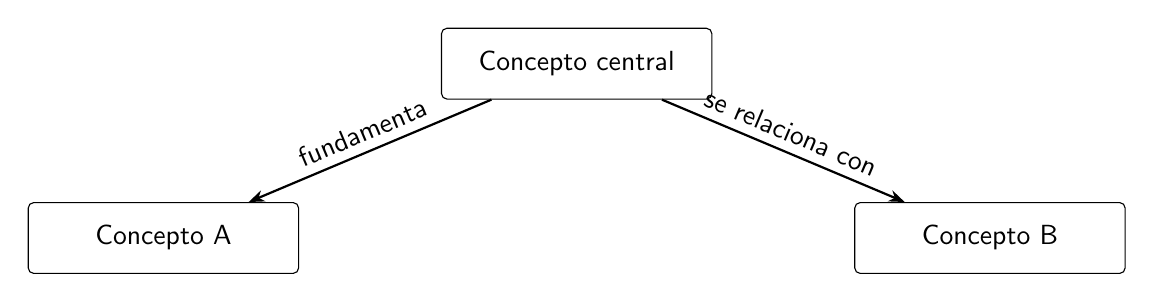
\begin{tikzpicture}[
  concepto/.style={rectangle, draw, rounded corners=2pt,
    align=center, text width=3.2cm, minimum height=0.9cm},
  flecha/.style={-{Stealth[length=2mm]}, thick}
]
\node[concepto] (a) {Concepto central};
\node[concepto, below left=1.3cm and 1.8cm of a] (b) {Concepto A};
\node[concepto, below right=1.3cm and 1.8cm of a] (c) {Concepto B};
\draw[flecha] (a) -- node[above, sloped]{fundamenta} (b);
\draw[flecha] (a) -- node[above, sloped]{se relaciona con} (c);
\end{tikzpicture}
\caption{Mapa conceptual de [tema]}
\end{figure}
\end{verbatim}

\subsubsection*{Línea de tiempo}

\begin{verbatim}
\begin{figure}[H]
\centering
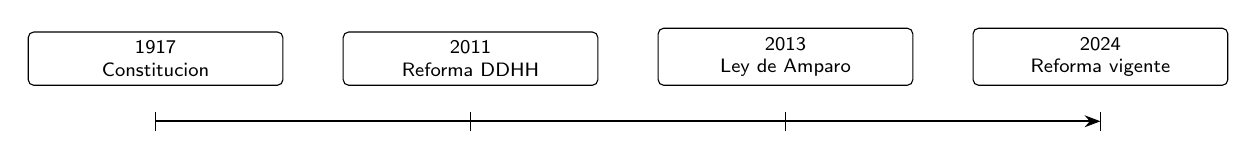
\begin{tikzpicture}[
  evento/.style={rectangle, draw, rounded corners=2pt,
    align=center, text width=3cm, font=\scriptsize},
  eje/.style={-{Stealth[length=2mm]}, thick}
]
\draw[eje] (0,0) -- (12,0);
\foreach \x/\anio/\texto in {
  0/1917/Constitucion,
  4/2011/Reforma DDHH,
  8/2013/Ley de Amparo,
  12/2024/Reforma vigente}
{
  \draw (\x,0.12) -- (\x,-0.12);
  \node[evento, above=0.45cm] at (\x,0) {\anio\\\texto};
}
\end{tikzpicture}
\caption{Linea de tiempo de [tema]}
\end{figure}
\end{verbatim}

\subsubsection*{Diagrama de flujo}

\begin{verbatim}
\begin{figure}[H]
\centering
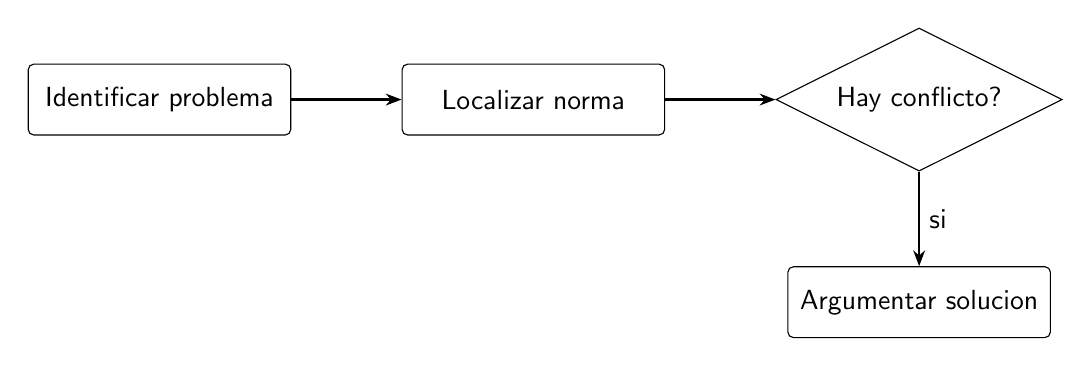
\begin{tikzpicture}[
  paso/.style={rectangle, draw, rounded corners=2pt,
    align=center, text width=3.1cm, minimum height=0.9cm},
  decision/.style={diamond, draw, aspect=2, align=center,
    text width=2.8cm, inner sep=1pt},
  flecha/.style={-{Stealth[length=2mm]}, thick}
]
\node[paso] (inicio) {Identificar problema};
\node[paso, right=1.4cm of inicio] (norma) {Localizar norma};
\node[decision, right=1.4cm of norma] (decision) {Hay conflicto?};
\node[paso, below=1.2cm of decision] (analisis) {Argumentar solucion};
\draw[flecha] (inicio) -- (norma);
\draw[flecha] (norma) -- (decision);
\draw[flecha] (decision) -- node[right]{si} (analisis);
\end{tikzpicture}
\caption{Diagrama de flujo de [proceso]}
\end{figure}
\end{verbatim}

\subsection{Cierre operativo}

La elección de una técnica no debe ser decorativa. Si la actividad pide un producto, la técnica funciona como una herramienta de análisis. El criterio de calidad es que el producto permita ver una decisión intelectual: qué se seleccionó, cómo se organizó, qué relación se construyó y qué postura se puede defender a partir de esa organización.


% ==============================================================================
% REFERENCIAS
% Reglas:
% - Toda fuente citada en el texto debe estar en el .bib.
% - Toda cita debe tener clave correcta.
% - Usar fuentes de la planeacion y, si se complementa, que sean confiables.
% - En el cuerpo: \citep{clave}; no usar solo URLs sueltas.
% ==============================================================================
\bibliography{EticaMoralJuridica}

% FIN DEL DOCUMENTO
\end{document}
